% This is "sig-alternate.tex" V2.1 April 2013
% This file should be compiled with V2.5 of "sig-alternate.cls" May 2012
%
% This example file demonstrates the use of the 'sig-alternate.cls'
% V2.5 LaTeX2e document class file. It is for those submitting
% articles to ACM Conference Proceedings WHO DO NOT WISH TO
% STRICTLY ADHERE TO THE SIGS (PUBS-BOARD-ENDORSED) STYLE.
% The 'sig-alternate.cls' file will produce a similar-looking,
% albeit, 'tighter' paper resulting in, invariably, fewer pages.
%
% ----------------------------------------------------------------------------------------------------------------
% This .tex file (and associated .cls V2.5) produces:
%       1) The Permission Statement
%       2) The Conference (location) Info information
%       3) The Copyright Line with ACM data
%       4) NO page numbers
%
% as against the acm_proc_article-sp.cls file which
% DOES NOT produce 1) thru' 3) above.
%
% Using 'sig-alternate.cls' you have control, however, from within
% the source .tex file, over both the CopyrightYear
% (defaulted to 200X) and the ACM Copyright Data
% (defaulted to X-XXXXX-XX-X/XX/XX).
% e.g.
% \CopyrightYear{2007} will cause 2007 to appear in the copyright line.
% \crdata{0-12345-67-8/90/12} will cause 0-12345-67-8/90/12 to appear in the copyright line.
%
% ---------------------------------------------------------------------------------------------------------------
% This .tex source is an example which *does* use
% the .bib file (from which the .bbl file % is produced).
% REMEMBER HOWEVER: After having produced the .bbl file,
% and prior to final submission, you *NEED* to 'insert'
% your .bbl file into your source .tex file so as to provide
% ONE 'self-contained' source file.
%
% ================= IF YOU HAVE QUESTIONS =======================
% Questions regarding the SIGS styles, SIGS policies and
% procedures, Conferences etc. should be sent to
% Adrienne Griscti (griscti@acm.org)
%
% Technical questions _only_ to
% Gerald Murray (murray@hq.acm.org)
% ===============================================================
%
% For tracking purposes - this is V2.0 - May 2012

\documentclass{sig-alternate-05-2015}
\usepackage{graphicx}
\usepackage[usenames,dvipsnames]{color}
\usepackage{soul} 
\usepackage{booktabs}

\newcommand{\todo}[1]
  {{\scriptsize \textbf{\color{red} {#1}}}}


\graphicspath{ {} }


\begin{document}

% Copyright
\setcopyright{acmcopyright}
%\setcopyright{acmlicensed}
%\setcopyright{rightsretained}
%\setcopyright{usgov}
%\setcopyright{usgovmixed}
%\setcopyright{cagov}
%\setcopyright{cagovmixed}


% DOI
\doi{10.475/123_4}

% ISBN
\isbn{123-4567-24-567/08/06}

%Conference
%\conferenceinfo{PLDI '13}{June 16--19, 2013, Seattle, WA, USA}

%\acmPrice{\$0.00}

%
% --- Author Metadata here ---
\conferenceinfo{MSR}{2016 Austin, Texas USA}
%\CopyrightYear{2007} % Allows default copyright year (20XX) to be over-ridden - IF NEED BE.
%\crdata{0-12345-67-8/90/01}  % Allows default copyright data (0-89791-88-6/97/05) to be over-ridden - IF NEED BE.
% --- End of Author Metadata ---

\title{A Deeper Look into Bug Fixes: Patterns, Replacements, Deletions, and Additions}

%
% You need the command \numberofauthors to handle the 'placement
% and alignment' of the authors beneath the title.
%
% For aesthetic reasons, we recommend 'three authors at a time'
% i.e. three 'name/affiliation blocks' be placed beneath the title.
%
% NOTE: You are NOT restricted in how many 'rows' of
% "name/affiliations" may appear. We just ask that you restrict
% the number of 'columns' to three.
%
% Because of the available 'opening page real-estate'
% we ask you to refrain from putting more than six authors
% (two rows with three columns) beneath the article title.
% More than six makes the first-page appear very cluttered indeed.
%
% Use the \alignauthor commands to handle the names
% and affiliations for an 'aesthetic maximum' of six authors.
% Add names, affiliations, addresses for
% the seventh etc. author(s) as the argument for the
% \additionalauthors command.
% These 'additional authors' will be output/set for you
% without further effort on your part as the last section in
% the body of your article BEFORE References or any Appendices.

\numberofauthors{1} %  in this sample file, there are a *total*
% of EIGHT authors. SIX appear on the 'first-page' (for formatting
% reasons) and the remaining two appear in the \additionalauthors section.
%
\author{
% You can go ahead and credit any number of authors here,
% e.g. one 'row of three' or two rows (consisting of one row of three
% and a second row of one, two or three).
%
% The command \alignauthor (no curly braces needed) should
% precede each author name, affiliation/snail-mail address and
% e-mail address. Additionally, tag each line of
% affiliation/address with \affaddr, and tag the
% e-mail address with \email.
%
% 1st. author
\alignauthor
Mauricio Soto$^1$, Ferdian Thung$^2$, Chu-Pan Wong$^1$, Claire Le Goues$^1$, and David Lo$^2$\\
       \affaddr{$^1$School of Computer Science, Carnegie Mellon University, Pittsburgh, PA\\
       $^2$Singapore Management University, Singapore}\\
       \email{mauriciosoto@cmu.edu, \{ferdiant.2013,davidlo\}@smu.edu.sg, \{chupanw,clegoues\}@cs.cmu.edu} 
}
% There's nothing stopping you putting the seventh, eighth, etc.
% author on the opening page (as the 'third row') but we ask,
% for aesthetic reasons that you place these 'additional authors'
% in the \additional authors block, viz.
%\additionalauthors{Additional authors: John Smith (The Th{\o}rv{\"a}ld Group,
%email: {\texttt{jsmith@affiliation.org}}) and Julius P.~Kumquat
%(The Kumquat Consortium, email: {\texttt{jpkumquat@consortium.net}}).}
\date{February 2, 2016}
% Just remember to make sure that the TOTAL number of authors
% is the number that will appear on the first page PLUS the
% number that will appear in the \additionalauthors section.

\maketitle
\begin{abstract}
  Many implementations of research techniques that automatically repair software
  bugs target programs written in C. Work that targets Java often begins from, or at
  least compares to, direct translations of such techniques to a Java context.
  However, Java and C are very different languages, and so Java should be
  studied to inform understanding of how to translate existing approaches to target it.
  We conduct a large-scale study of bug-fixing commits
  to Java projects, focusing on assumptions underlying common
  search-based repair approaches.  We make observations that can be
  leveraged to guide high quality automatic software repair to target Java specifically,
  including common and uncommon statement replacements as conducted by human
  developers and the applicability of previously-proposed patch construction
  operators in the Java context. 
\end{abstract}


%
% The code below should be generated by the tool at
% http://dl.acm.org/ccs.cfm
% Please copy and paste the code instead of the example below. 
%
\begin{CCSXML}
<ccs2012>
 <concept>
  <concept_id>10010520.10010553.10010562</concept_id>
  <concept_desc>Computer systems organization~Embedded systems</concept_desc>
  <concept_significance>500</concept_significance>
 </concept>
 <concept>
  <concept_id>10010520.10010575.10010755</concept_id>
  <concept_desc>Computer systems organization~Redundancy</concept_desc>
  <concept_significance>300</concept_significance>
 </concept>
 <concept>
  <concept_id>10010520.10010553.10010554</concept_id>
  <concept_desc>Computer systems organization~Robotics</concept_desc>
  <concept_significance>100</concept_significance>
 </concept>
 <concept>
  <concept_id>10003033.10003083.10003095</concept_id>
  <concept_desc>Networks~Network reliability</concept_desc>
  <concept_significance>100</concept_significance>
 </concept>
</ccs2012>  
\end{CCSXML}


%
% End generated code
%

%
%  Use this command to print the description
%
\printccsdesc

% We no longer use \terms command
%\terms{Theory}

\keywords{Automatic error repair; Maintainability; Human-like patches}

\section{Introduction}

There has been considerable attention paid to automatic
program repair in recent
years~\cite{kim2013,legoues2012,pan2009,
  Mechtaev15,Long2016}.
%
One broad class of techniques in this space take a generate-and-validate
approach: \emph{generating} a large number of candidate patches using a
pre-defined set of mutation operators, and then \emph{validating} correctness with
respect to a set of test cases.  Mutation operators range from simple, coarse
granularity statement-level mutations to human-constructed templates learned
from a large corpus of previous human bug-fixing commits.

A considerable proportion of these works target programs written in C.
Indeed, researchers targeting Java often start from or compare against
Java-based implementations of techniques originally
implemented for C~\cite{nopol,kim2013}. % Even PAR~\cite{kim2013}, perhaps the
% best-known previously-proposed Java-based program repair technique, both starts
% from and is directly compared to a Java implementation of GenProg~\cite{genprog}, which
% targets the C programming language.  
%
This is an oversight because Java and C are very different languages.
Consider GenProg~\cite{legoues2012}, which
combines statement-level mutations into patches to address a particular
defect. Which ``Statements'' (a semantic unit in C) should be manipulated in Java?
Can we learn
intelligent rules to inform candidate modifications
(cf. Prophet~\cite{Long2016}, for C)?  What types of semantic scoping
should limit mutations, given the relative stringence of the Java
compiler?

In this paper, we study bug-fixing commits to Java programs, 
taken from several million human-made bug fixes from Github. We study broad
characteristics of these changes; the applicability of previously-proposed
Java repair templates~\cite{kim2013}; and the nature
of additions and replacements of Java statements in bug-fixing commits. We make
observations to directly guide future research in automatic repair of Java
programs, to increase the success rate of such techniques and the degree to
which the patches are human-like and therefore more readable and maintainable by
human developers. This is important, because patch quality is an important
concern in this area~\cite{Qi15}.

% On the other hand, some approaches~\cite{kim2013} search for specific patterns
% and modify source code according to predefined templates. A well known approach
% is PAR~\cite{kim2013}, which creates 10 different repair templates and applies
% them to the buggy code in an effort to repair it. In this paper we have taken 8
% out of the 10 PAR templates and tested how common they are in the repairs made
% by programmers in the latest official data dump of Github as of September 2015
% provided by~\cite{dyer2013}.  Our results provide evidence of how common those
% patterns are in practice. We take as reference the study performed by Dongsun
% Kim et al.~\cite{kim2013} in which they look for the most common ways in which
% programmers patch bugs in software. The researchers developed a variation of the
% tool Genprog~\cite{weimer2009,legoues2012} with several different templates
% resembling patterns programmers use to patch bugs, and then performed an
% empirical study to evaluate which patches do human programmers prefer.

\vspace{1ex} \noindent\textbf{Related work.} Zhong and Su~\cite{zhong2015} study
a similar set of questions in 5 projects. In this paper we have studied a much
larger dataset~\cite{dyer2013} with 380,125 repositories; we have studied more
statement types, and we have studied replacements, omitted from Zhong and Su's
analysis. Similar to our study in Section~\ref{sec:stmtstudy}, researchers have
studied AST-level changes~\cite{Martinez:2015ez} or line
changes~\cite{Asaduzzaman:2013gu, Asaduzzaman:2013df} across bug fixing commits.
Although granularity differs, our approach is novel with respect to scale of
analysis. Barr et al.~\cite{Barr14fse} studied changes to Java programs to
understand the ``Plastic Surgery Hypothesis'' underlying certain types of
program repair, an orthogonal concern. Kim et al.~\cite{kim2013} manually
analyze changes to Java programs to inform an automated repair technique, and
show that doing so results in higher-quality repairs; we study their templates
heuristically on a different dataset. Their results motivate studies of human
repairs, as it may result in better patches.  Long and Rinard learn
probabilistic models from bug fixes to C code~\cite{Long2016}. Our analysis is
significantly less precise and does not inform a new technique.  Rather, it
serves as a starting point for research on the repair of Java bugs.

\section{Dataset and Characteristics}

First, we broadly characterize bug-fixing commits to Java code.  In this paper,
we study the \emph{September 2015/Github} dataset on Boa, including $7,830,023$
Java projects with $23,229,406$ revisions. Boa identifies $4,590,679$ as bug
fixing.

\vspace{1ex}
\noindent\textbf{How many files are changed to fix a bug?}
%

We consider a file changed if it is new, modified, or deleted in a commit. In
total, $52,052,571$ files were changed, an average of $11.3$ files per
bug-fixing commit, and the median number is $2$.  Although the median number
conforms to our intuition, the average is surprisingly high: most automatic
program repair techniques assume that bugs are local.  We hypothesize several
explanations: Other software artifacts (e.g.  documentation) may be updated
after bug  fixing, or fixing commits may contain changes unrelated to fixing
the bug (e.g.  refactoring, feature addition).  To better understand this
phenomenon, we ask:

\begin{table}
\centering
  \begin{tabular}{ l | r  r }
  \toprule
  File Kind & Total & Average \\ 
  \midrule
  Binary & 752,945 & 0.16 \\ 
  Java (ERROR) & 2,073,558 & 0.45 \\ 
  Java (JLS2) & 2,607,413 & 0.57 \\ 
  Java (JLS3) & 15,748,967 & 3.43 \\
  Java (JLS4)  & 83,798 & 0.02 \\ 
  Text & 541,023 & 0.12 \\ 
  XML & 6,818,299 & 1.49 \\ 
  UNKNOWN & 23,426,568 & 5.10 \\ 
\bottomrule
  \end{tabular}
  \caption{File Types of Changed Files}
  \label{tbl:fileType}
\end{table}
\vspace{1ex}
\noindent\textbf{What are the types of those changed files?}
%
To answer this question, we iterate over all changed files in each bug fixing
revision and count the total number for each file type. Results are shown in
Table~\ref{tbl:fileType}.
%

JAVA (ERROR) files are those that Boa failed to parse. JLS2, JLS3, and JLS4
represent Java files written in different J2SE versions.  We see that text and
binary files are changed least frequently. This is unsurprising, since text
files are often documentation, and binaries should be changed rarely. If we
consider all 4 kinds of Java files as one kind, on average, each bug fixing
revision changes $4.47$ Java files. This does not conform to our assumption of
bug locality. XML files in Java projects usually represent build files;
changing build files is unsurprising.  Rather more surprising is how frequently
UNKNOWN files are changed. Given that all projects are Java projects, it is
unclear whether these are written in other programming languages. We
hypothesize they might be test resources.  To better understand what changes
are usually made to Java files, we next ask:

\vspace{1ex}
\noindent\textbf{How often do developers introduce new classes, methods, fields,
	local variables in
bug fixing commits?} 
%
This question is interesting because most automatic program repair approaches
do not create methods or variable declarations, nor do most explicitly consider
object-oriented features, like fields or classes. 

Table~\ref{tbl:new} shows that introducing new
classes and new variables is rare. On average, we still have $0.69$ new methods
per bug fix. These methods naturally contain new test methods (annotated by
@Test, for example), which is not too alarming. However,
what surprises us is that $1.32$ fields are created per bug fix.  This indicates
that automatic program repair approaches should pay attention to the state of
the class when fixing Java programs.

\begin{table}
\centering
  \begin{tabular}{l | r  r }
  \toprule
  Introducing & Total Number & Average \\ \midrule
  Class & 729,201 & 0.16 \\ 
  Methods & 3,186,867 & 0.69 \\ 
  Fields & 6,076,646 & 1.32 \\ 
  Variables & 924,259 & 0.2 \\ 
\bottomrule
  \end{tabular}
  \caption{Introducing new classes, methods, fields, local variables to fix bugs}
  \label{tbl:new}
\vspace{-0.5cm}
\end{table}


\section{Bug Fixing Patterns}\label{sec:method}

One of the best-known program repair techniques to target Java is
PAR~\cite{kim2013}.  PAR
modifies Java code according to predefined templates, constructed by humans
to cover a large set of bug fixes from an existing corpus.  These templates provide
important source of possible 
mutations to study to inform future directions. 
We therefore search for most of the PAR bug fixing patterns,
estimating their prevalence in this
dataset.

% A well known approach
% is PAR~\cite{kim2013}, which creates 10 different repair templates and applies
% them to the buggy code in an effort to repair it. In this paper we have taken 8
% out of the 10 PAR templates and tested how common they are in the repairs made
% by programmers in the latest official data dump of Github as of September 2015
% provided by~\cite{dyer2013}.  Our results provide evidence of how common those
% patterns are in practice. We take as reference the study performed by Dongsun
% Kim et al.~\cite{kim2013} in which they look for the most common ways in which
% programmers patch bugs in software. The researchers developed a variation of the
% tool Genprog~\cite{weimer2009,legoues2012} with several different templates
% resembling patterns programmers use to patch bugs, and then performed an
% empirical study to evaluate which patches do human programmers prefer.

\subsection{Detecting PAR templates using Boa}

Boa's capabilities are powerful, but limited in the precision it enables in
our detection of PAR bug-fixing patterns. For example, it cannot directly \texttt{diff}
two files versions. Thus, rather than finding the exact count of
bug fixing patterns, we approximate by processing pre- and
post-fix files separately.  Additionally, there are
two of the 10 patterns that cannot be easily detected by
Boa, as we describe below. 
%
The patterns we search for are as follows, including our mechanism for
detecting them:

\vspace{1ex}
\noindent {\bf Altering method parameters (AMP)}.  This template changes 
input method parameters. %(\texttt{obj.method(v1,v2) $\rightarrow$
%obj.method(v1,v3)}). 
To detect this pattern, for both pre- and post-fix versions
of a buggy file, we create a custom method call signature that
contains the name string, literal parameters string, and variable parameters string (complex
expressions are listed as ``OTHER'' string).
%  This is due to inexistence of
% function that can print Abstract Syntax Tree (AST) back to source code in
% Boa. 
We discard method signatures that appear both in pre- and post-fix
versions, and then identify methods with the same name and the
same number of parameters, but different signatures between versions. 

\vspace{1ex}
\noindent {\bf Calling another method with the same parameters (MSM)}.  This
template changes a method name. % (\texttt{obj.method1(param) $\rightarrow$
%obj.method2(param)}).  
To detect it, we create a method signature similar
to the above for AMP, looking for methods
with the exact same parameter signature but different names in pre- and
post-fix versions. %If it exists, we consider that MSM pattern is found.

\vspace{1ex}
\noindent
{\bf Calling another overloaded method with one more parameter (COM)}. This
template adds a parameter to a method. %(\texttt{obj.method(v1) $\rightarrow$ obj.method(v1,v2)}).
We create a method signature similar to the above, seeking methods with
  the same name, but with one more parameter in the post-fix version. 

\vspace{1ex}
\noindent
 {\bf Add or remove a branch condition (ABC)}. This template adds or removes a condition.
%(e.g., \texttt{if(a != b) $\rightarrow$ if(a != b \&\& c == 0)}).
We count the number of { \em logical and} and {\em
    logical or} inside if conditional expression for both pre- and post-fix
  version. We assume that the addition/removal of logical operators indicate
  addition/removal of condition. If there is a count difference between pre- and post-fix version,
  we consider an instance of the ABC pattern is found. 

\vspace{1ex}
\noindent
{\bf Initializing an object (IAO)}. This template adds a initialization to object
declaration.  We count the number of NEW expressions in variable declarations
for both pre- and post-fix versions. If there is a larger count in post-fix
version, we consider that an instance of the IAO pattern is found.

\vspace{1ex}
\noindent
 {\bf Adding a null checker (ANC)}.  This template inserts a condition to check whether an
    object is null.
%	{\bf Example:} obj.m1() $\rightarrow$ if(obj!=null){obj.m1()}
  To detect ANC pattern, we count the number of if conditional expressions that
  contains {\em !=null} or {\em ==null} for both pre- and post-fix
  version. If there is a larger count in post-fix version,
  we consider that an instance of the ANC pattern found.

\vspace{1ex}
\noindent
 {\bf Adding an array out of bound checker (AOB)}. This pattern inserts a condition to check that an array
    index is within bound right before the index is used.
%	{\bf Example:} arr[idx]=0 $\rightarrow$ if(idx<arr.length){arr[idx]=0}.
 We count the number of if conditional expression that
  contains {\em expr<var.length} or {\em var.length>expr} for both pre- and
  post-fix version. If there is a larger count in post-fix version, we consider that an instance of the AOB pattern is found.

\vspace{1ex}
\noindent
 {\bf Adding a collection out of bound checker (COB)}.  This pattern inserts a condition to check that a
    collection index is within bound before it is used.
To detect COB pattern, we count the number of if conditional expression that
contains {\em expr<col.size()} or {\em col.size()>expr} for both pre- and
post-fix version. If the is a larger count in post-fix
version, we consider that an instance of the COB pattern is found.

\vspace{1ex} The above patterns cover 8 out of 10 bug fixing patterns in
PAR. The other two patterns are (1) Class Cast Checker (cannot be analyzed because
Boa does not support the {\em instanceof} expression); and (2) Expression Changer (requires us to track scope between pre- and post-fix version; not
easily supported by Boa). Investigating 8 out of
10 patterns still shows us how common the patterns actually are.

\subsection{Results} \label{sec:freqfixpattern}

\begin{table}[!htb]
	\centering
	\begin{tabular}{lrr} 
		\hline
		& \textbf{\#Appearance} & \textbf{Percentage}\\
		\hline
		%Buggy Files & 46,301,429 \\ 
		AMP Pattern & 901,083 & 1.95\%\\
		MSM Pattern & 783,073 & 1.69\%\\
		COM Pattern & 270,128 & 0.58\%\\ 
		ABC Pattern & 1,959,377 & 4.23\%\\  
		IAO Pattern & 1,308,006 & 2.82\%\\  
		ANC Pattern & 1,340,561 & 2.90\%\\  
		AOB Pattern & 128,016 & 0.28\%\\  
		COB Pattern & 262,915 & 0.57\%\\   
		\hline
	\end{tabular}
	\caption{Frequency of Bug Fixing Patterns}\label{tab:freqpattern}
	
\end{table}


Table~\ref{tab:freqpattern} estimates the prevelance of PAR templates in the
Java dataset. The most common pattern we observed is ABC (add or remove a branch condition); and the least common
pattern is AOB (adding an array out of bound checker). If we conservatively assume that these patterns never appear together, they
cover 14.78\% of buggy files. In the dataset studied by Kim et al., the overall
10 patterns cover almost 30\% of real patches~\cite{kim2013}. Although we only analyze 8
out of 10 bug fixing patterns, it is unlikely the final two will cover the
difference. To even get close to 30\%, each of the patterns need to cover around 7\% of buggy files and we are still assuming that the patterns never appear together. 
%Moreover, our detection is imprecise, and might represent an upper bound. 
This suggests that these fixing patterns might not generalize
beyond an initial dataset, and that more work remains to expressively characterize human bug-fixing behavior.



\section{Statement-level mutations}\label{sec:stmtstudy}
\begin{table*}
	\centering
	\resizebox{\textwidth}{!}{
	%\renewcommand{\arraystretch}{0.9}% Tighter
		\begin{tabular}{l|rrrrrrrrrrrrrrr} \toprule
			&\texttt{Assert}&\texttt{Break}&\texttt{Continue}&\texttt{Do}&\texttt{For}&\texttt{If}&\texttt{Label}&\texttt{Return}&\texttt{Case}&\texttt{Switch}& \texttt{Synch}&\texttt{Throw}&\texttt{Try}&\texttt{TypeDecl}&\texttt{While}
			\\ \midrule
			
\texttt{Assert}	&-&7.48&3.76&0.53&8.30&23.05&0.31&20.04&4.90&4.62&1.30&13.50&7.23&0.03&4.95
\\
\texttt{Break} &1.00&-&4.08&0.60&9.93&26.03&0.13&25.39&2.48&1.57&1.79&8.39&11.73&0.10&6.77
\\
\texttt{Continue} &1.74&9.42&-&1.28&11.39&18.25&0.35&22.60&3.80&2.85&2.17&8.98&9.42&0.11&7.63
\\
\texttt{Do} &0.81&5.26&6.60&0.00&9.44&14.21&0.18&15.86&3.73&1.67&1.97&5.88&6.39&0.03&27.98
\\
\texttt{For} &0.86&6.28&3.19&0.79&-&22.89&0.09&21.08&5.01&3.34&1.87&10.01&10.71&0.08&13.79
\\
\texttt{If}&1.64&8.43&2.87&0.60&13.49&-&0.24&26.46&7.45&4.80&2.85&9.89&15.11&0.08&6.11
\\
\texttt{Label} &1.30&8.33&7.86&1.11&5.18&22.85&-&15.17&3.05&2.04&14.62&10.45&4.16&0.09&3.79
\\
\texttt{Return} &1.13&9.41&3.11&0.49&13.33&27.24&0.24&-&5.59&3.65&2.55&14.91&12.61&0.12&5.61
\\
\texttt{Case} &0.78&2.84&2.84&0.39&10.27&31.79&0.16&22.40&-&0.46&2.07&7.37&11.69&0.08&6.87
\\
\texttt{Switch}&1.14&2.72&3.80&0.55&11.07&34.14&0.13&21.86&0.75&-&1.53&8.65&9.02&0.05&4.58
\\
\texttt{Synch} &0.80&6.57&2.28&0.43&10.21&24.18&0.05&19.77&6.35&2.07&-&9.16&12.16&0.04&5.93
\\
\texttt{Throw} &2.11&6.57&2.58&0.48&11.87&18.84&0.17&32.28&4.64&3.30&2.74&-&10.08&0.07&4.27
\\
\texttt{Try}&0.71&7.41&3.02&0.66&11.73&27.75&0.11&23.24&5.63&2.65&2.58&8.99&-&0.09&5.42
\\
\texttt{TypeDecl} &0.00&4.51&7.52&1.00&10.28&21.05&0.50&17.79&6.02&1.75&2.01&9.27&11.53&-&6.77
\\
\texttt{While}& 0.72&8.02&3.82&1.96&23.16&19.78&0.12&16.48&6.56&3.09&1.64&6.81&7.80&0.04&-
			\\ \bottomrule
		\end{tabular}
		}
		\caption{Likelihood of replacing a statement type (row) by a statement of
          another type (column), for Java.}\label{tab:likeliness}
\end{table*}

\begin{figure*}[!t] \centering 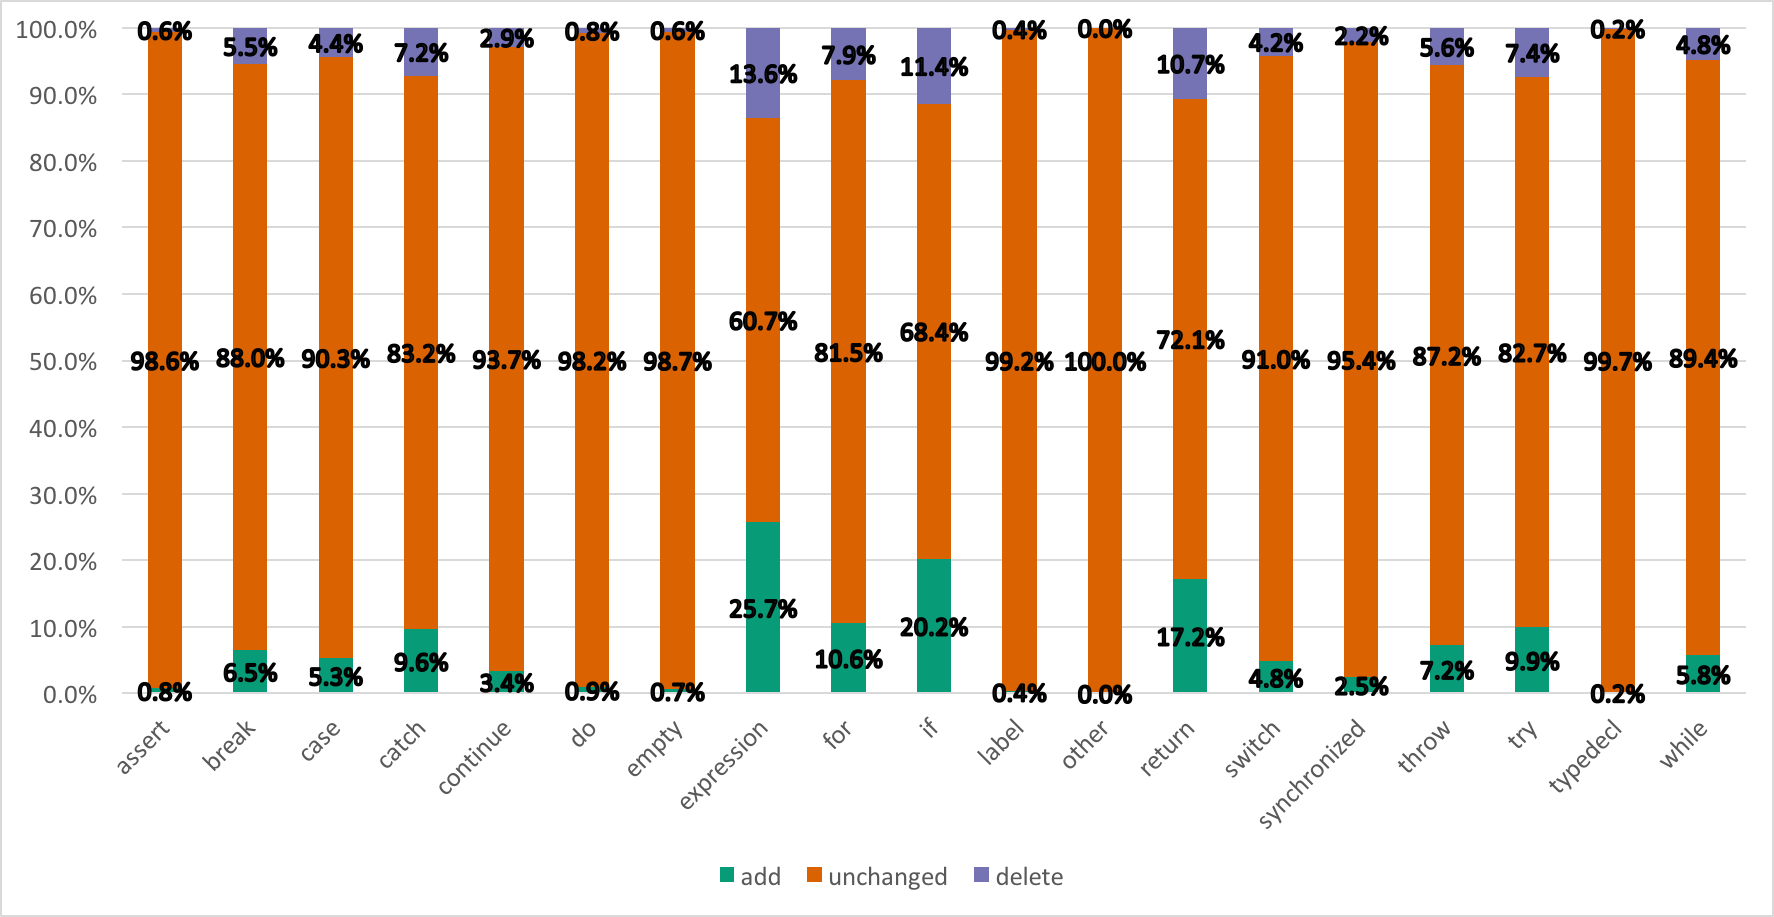
\includegraphics[width=\textwidth]{StmtType}
	\vspace{-0.7cm} \caption{For each kind of statement, how many
	bug fixing revisions add/delete statements of the same kind?}
	\label{fig:StmtType} \end{figure*}


Some automatic program repair approaches seek generality by using
higher-granularity mutation operators such as statement-level addition, deletion and replacement. To
support the generation of high-quality patches, we 
next analyze how developers mutate source code to fix bugs at this granularity
level. 

\subsection{Detection Approach}
Because direct diffs are difficult to identify on this dataset, we heuristically approximate the
extent to which one statement type appears to be ``replaced'' by another.
For each modified file, we count the number of
appearances of each statement type in the file pre- and post-commit.  We then
compare the results to see how many of each statement type was removed, and how
many inserted, to roughly characterize the types of replacement that happen at a
per-file level.
%   For each statement type (as tagged by the Boa infrastructure
% for Java), we process the results as follows: if number of occurrences of one
% statement type decreased post-fix and the number of another type increased, we
% say that the first statement type was replaced by the second statement type for
% that file. 
Note that this analysis doesn't distinguish the
replacement of the same statement kind, since we are counting the amount of
appearances of each statement kind.

We follow a similar approach to approximate a count of deletions and
insertions. 
For each bug fixing revision $r$ and each statement kind $k$, we count how many
statements of kind $k$ are there in revision $r$ and $r-1$ ($r-1$ means the
revision before revision $r$), and then compare the two numbers. 

\subsection{Results}

\noindent\textbf{Potential replacements.} Table~\ref{tab:likeliness} shows
the replacement likelihood for our dataset 
(each cell shows the percent of the time that the statement in the \emph{row}
was replaced by a statement of the type in the \emph{column}). For example, if
the cell in the Do statement row (row 5) and Assert statement column (column 2)
shows 0.81, it means that Do statements were
replaced by Assert statements 0.81\% of the times.

Additional results (raw numbers not shown) show that the most common replacement
is replacing Return statement with If statement (appearing in 30,489 files). The
second most common replacement is replacing an If statement with a Return
statement, which had 28,536 appearances. 
By contrast, the least common replacement was an Assert
statement replacing a Type Declaration statement, which we did not observe. 
The second least common replacement was a Do statement for a Type
Declaration or a Label with a Type; we observed these once each.  

The most common
\emph{replacer} statement kind (the statement kind that most commonly replaces
others) is the \texttt{If Statement} (101,366 appearances). The least
common \emph{replacer} is the \texttt{Type Declaration Statement} with 447
appearances.
The most common \emph{replacee} was the
\texttt{Return Statement} with 111,938 appearances; and the least common
\emph{replacee} was the \texttt{Type Declaration}, with 399 appearances.


\vspace{1ex}
\noindent \textbf{Potential deletions and insertions} From Figure~\ref{fig:StmtType}, we
can see that, expression, if, return, for and try catch statements are added
most often. Meanwhile, the same types of statements are also deleted most
often. This finding indicates that most bugs were fixed by changing the control
flow of the program.

An important study that complements for our study is the repair model approach
proposed by Martinez and Monperrus~\cite{Martinez:2015ez}, in which they discuss
a probability distribution for when to apply which kind of edit. Although their
approach is able to trace more fine-grain AST-level changes, our results are
consistent with their findings. For example, their empirical
analysis~\cite{Martinez:2015ez} shows that method invocations, if statements,
and variable declaration statements are added/deleted/updated most often, which
is also illustrated in Figure~\ref{fig:StmtType} (In Boa, method invocation and
variable declaration fall into the category of expression). It is also worth
mentioning that their study covers 14 repositories with 89,993 versioning
transactions, while our study studies 380,125 repositories with 23,229,406
revisions. 

\section{Discussion}

\noindent\textbf{Threats to validity.} Since we are using a DSL
provided by Boa, the correctness of our analysis
depends on both our programs and Boa itself. For example, we rely on Boa to
identify bug fixing revisions; however, precisely accomplishing this is an open
problem.  To mitigate the risk of errors in
implementation, we open source our scripts\footnote{\url{https://github.com/chupanw/BoaChallenge}}.
Because Boa does not provide an easy mechanism
to identify precise, statement-level diffs between revisions, our template
matching and analysis of code changes (by counting each statement kind) only
provide estimates of behavior; we consider our results as informative
approximations. 

The findings of our study provide useful insights for automatic program repair
tools in Java. It suggests that patterns proposed by the state-of-the-art in
generate and validate bug report for Java are insufficient cover the extent of
bug fixes in our dataset.  Adding more patterns is one solution, but may not be
a general one.  Our findings further suggest that
mutation based program repair may need to consider field or method insertion to
achieve human-comparability in patches.  A deeper look suggests that such
techniques may benefit from leveraging probabilistic knowledge of what types of
statements are commonly inserted, deleted, or replaced in Java bug-fixing commits.
Overall, our findings motivate additional study of 
repair in Java, as assumptions that underlie approaches that target C seem
unlikely to translate directly.

% demonstrate that our knowledge of bug fixing
% properties in Java is still lacking and therefore more research on it are
% warranted.

%   We studied the applicability of the state-of-the-art in
% mutation operators to this dataset, 
% showing that 8 out of 10 bug fixing patterns in PAR cover only 15\% of bug
% fixes in this dataset.  Finally, investigated statement level mutations and
% summarized the likelihood of statement insertion, deletion, and replacement.
% These results suggest 

% This study is directly applicable to automatic software repair. Most common
% tools for automatic software repair~\cite{kim2013,legoues2012} first localize a
% defect and then randomly select edits to 
% find a faulty statement using several different fault localization
% techniques~\cite{fry2010}, and once they have that faulty statement, they apply
% different kinds of edits to it, usually at random. Which makes it equally likely
% to replace an statement for another without looking at the kinds of statements
% being replaced. With this study, we are able to make a more accurate guess based
% on the phenomenon we observed from Table~\ref{tab:likeliness} and
% Figure~\ref{fig:StmtType}.

% For example, if we are fixing a Java program, and we have a faulty statement
% that happens to be a For Statement. Then we can look for the most likely
% statements to replace a For Statement (row 6): If statement (22.89\%
% likeliness), Return statement (21.08\%), and a While statement (13.79\% of
% likeliness to replace a For Statement). We also know that there is a 7.9\% of
% cases in which human programmers deleted this kind of statement, and in 10.6\%
% of the cases, a For statement was added to patch a bug. This way we provide
% guidelines to the automatic bug repair approaches to consider this on their
% effort to find a patch.




%\end{document}  % This is where a 'short' article might terminate



\bibliographystyle{abbrv}
\bibliography{sigproc}  % sigproc.bib is the name of the Bibliography in this case
% You must have a proper ".bib" file
%  and remember to run:
% latex bibtex latex latex
% to resolve all references
%
% ACM needs 'a single self-contained file'!
%
%APPENDICES are optional
%\balancecolumns


%\balancecolumns % GM June 2007
% That's all folks!
\end{document}
